\documentclass{standalone}
\usepackage{tikz}
\usetikzlibrary{patterns, positioning}
\usepackage[sfdefault]{ClearSans} %% option 'sfdefault' activates Clear Sans as the default text font
\usepackage[T1]{fontenc}

\begin{document}
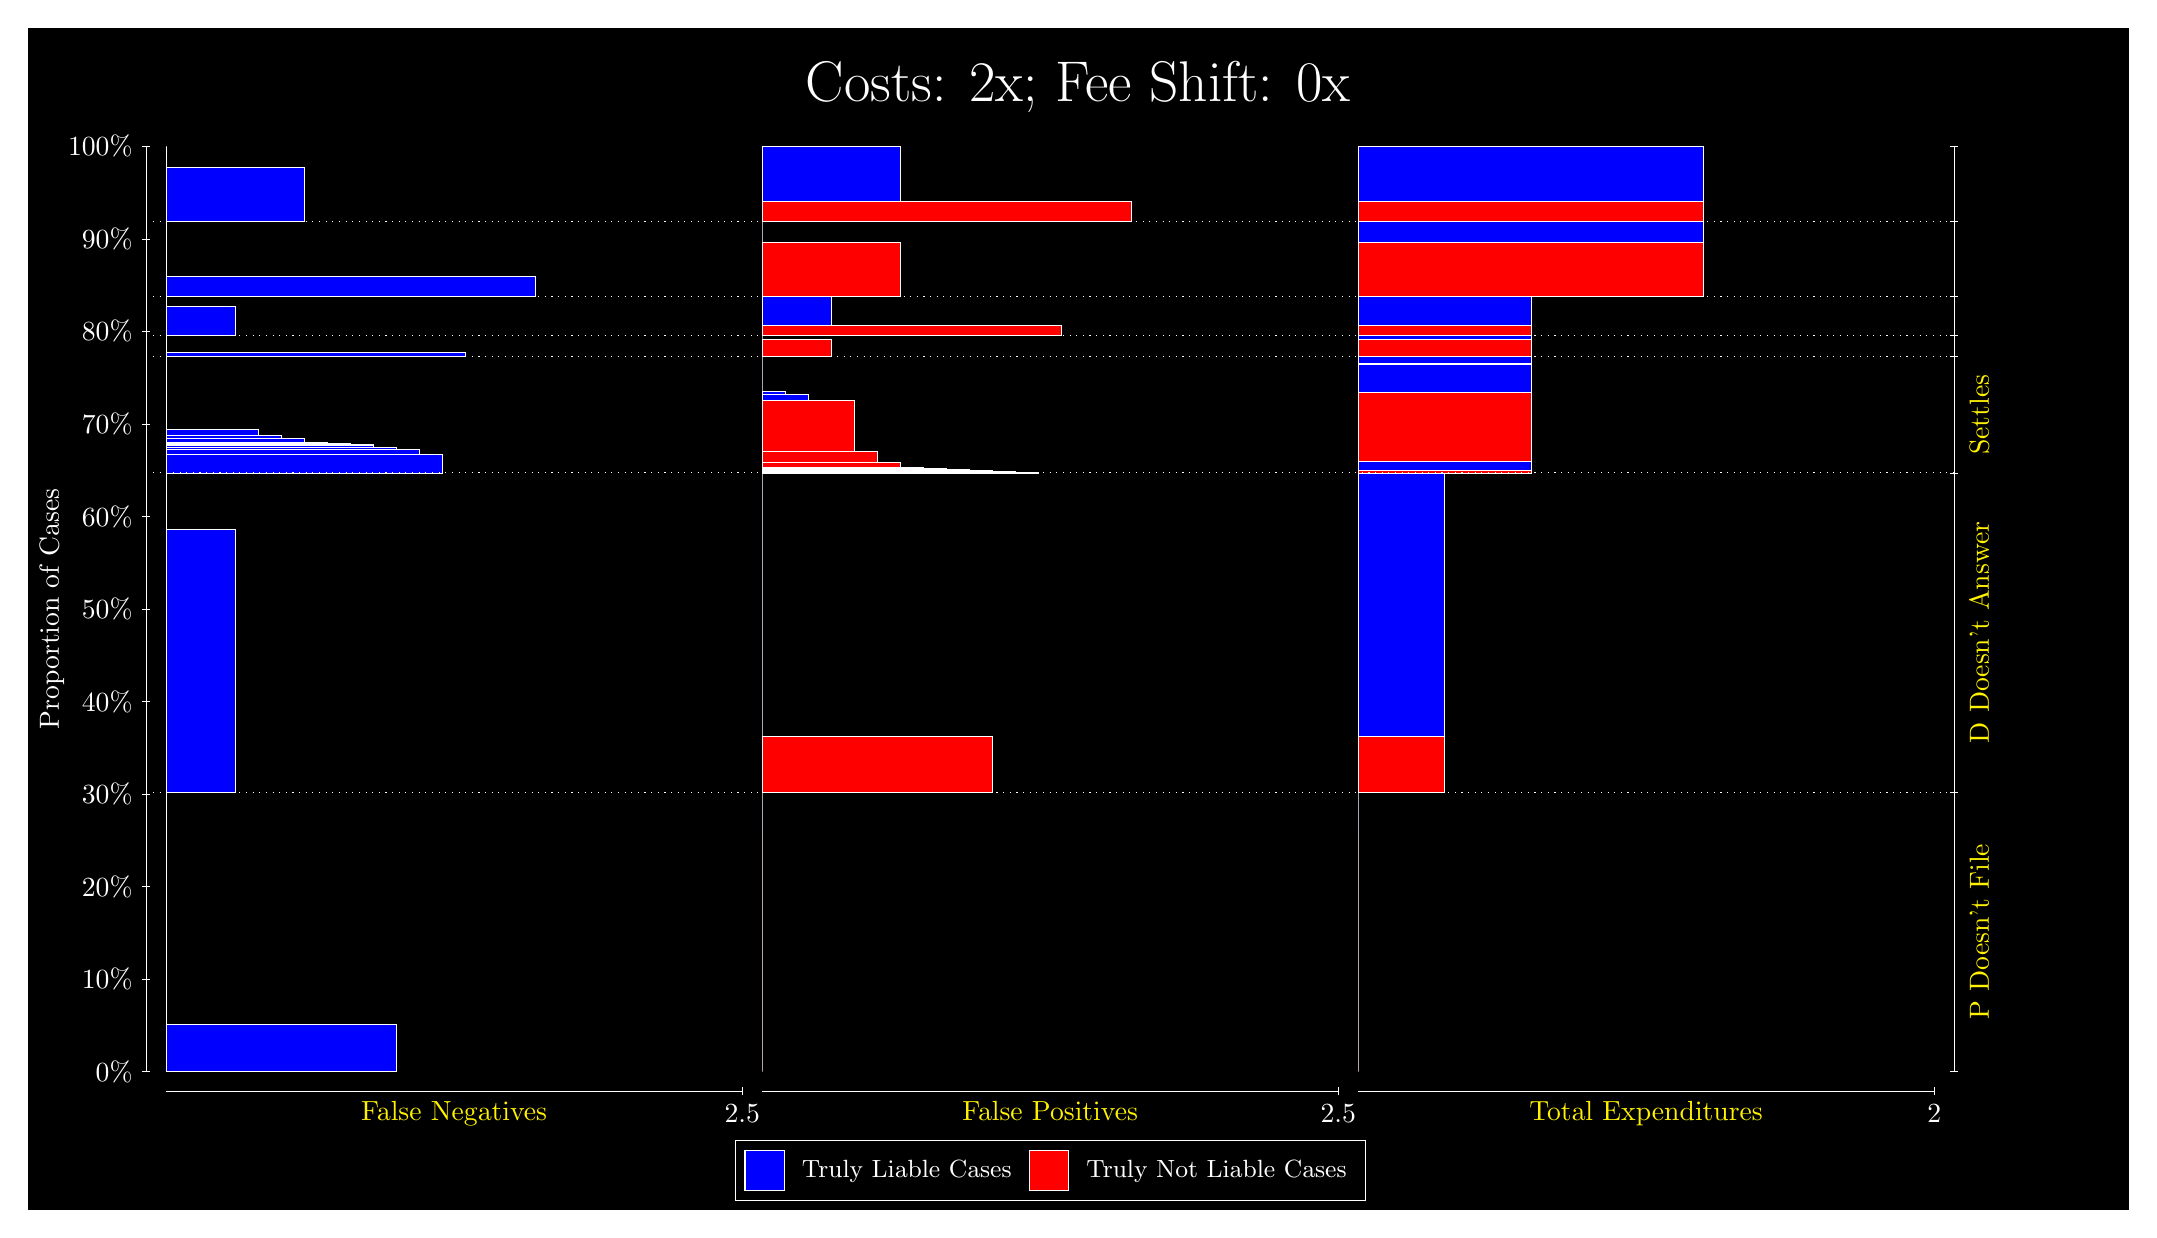
\begin{tikzpicture}
\draw[fill=black] (0,0) rectangle (26.667,15);
\draw[text=white] (0,13.5) rectangle (26.667,15) node[midway] {\huge Costs: 2x; Fee Shift: 0x};
\draw[white, very thin] (1.5,1.75) -- (1.5,13.5);
\node[rotate=90, text=white, anchor=center] at (0.3, 7.625) {Proportion of Cases};
\draw[white, very thin] (1.45,1.75) -- (1.55,1.75);
\node[text=white, anchor=east] at (1.45, 1.75) {0\%};
\draw[white, very thin] (1.45,2.925) -- (1.55,2.925);
\node[text=white, anchor=east] at (1.45, 2.925) {10\%};
\draw[white, very thin] (1.45,4.1) -- (1.55,4.1);
\node[text=white, anchor=east] at (1.45, 4.1) {20\%};
\draw[white, very thin] (1.45,5.275) -- (1.55,5.275);
\node[text=white, anchor=east] at (1.45, 5.275) {30\%};
\draw[white, very thin] (1.45,6.45) -- (1.55,6.45);
\node[text=white, anchor=east] at (1.45, 6.45) {40\%};
\draw[white, very thin] (1.45,7.625) -- (1.55,7.625);
\node[text=white, anchor=east] at (1.45, 7.625) {50\%};
\draw[white, very thin] (1.45,8.8) -- (1.55,8.8);
\node[text=white, anchor=east] at (1.45, 8.8) {60\%};
\draw[white, very thin] (1.45,9.975) -- (1.55,9.975);
\node[text=white, anchor=east] at (1.45, 9.975) {70\%};
\draw[white, very thin] (1.45,11.15) -- (1.55,11.15);
\node[text=white, anchor=east] at (1.45, 11.15) {80\%};
\draw[white, very thin] (1.45,12.325) -- (1.55,12.325);
\node[text=white, anchor=east] at (1.45, 12.325) {90\%};
\draw[white, very thin] (1.45,13.5) -- (1.55,13.5);
\node[text=white, anchor=east] at (1.45, 13.5) {100\%};

\draw[white, very thin] (24.457,1.75) -- (24.457,13.5);
\draw[white, very thin] (24.407,1.75) -- (24.507,1.75);
\node[anchor=west] at (24.407, 1.75) {};
\draw[white, very thin] (24.407,5.2987) -- (24.507,5.2987);
\node[anchor=west] at (24.407, 5.2987) {};
\draw[white, very thin] (24.407,9.3537) -- (24.507,9.3537);
\node[anchor=west] at (24.407, 9.3537) {};
\draw[white, very thin] (24.407,10.829) -- (24.507,10.829);
\node[anchor=west] at (24.407, 10.829) {};
\draw[white, very thin] (24.407,11.103) -- (24.507,11.103);
\node[anchor=west] at (24.407, 11.103) {};
\draw[white, very thin] (24.407,11.592) -- (24.507,11.592);
\node[anchor=west] at (24.407, 11.592) {};
\draw[white, very thin] (24.407,12.542) -- (24.507,12.542);
\node[anchor=west] at (24.407, 12.542) {};
\draw[white, very thin] (24.407,13.5) -- (24.507,13.5);
\node[anchor=west] at (24.407, 13.5) {};

\draw[white, very thin, fill=blue] (1.75,1.75) rectangle (4.6775,2.3463);
\draw[white, very thin, fill=red] (1.75,2.3463) rectangle (1.75,5.2987);
\draw[white, very thin, fill=blue] (1.75,5.2987) rectangle (2.6283,8.6413);
\draw[white, very thin, fill=red] (1.75,8.6413) rectangle (1.75,9.3537);
\draw[white, very thin, fill=blue] (1.75,9.3537) rectangle (5.2631,9.5919);
\draw[white, very thin, fill=blue] (1.75,9.5919) rectangle (4.9703,9.6523);
\draw[white, very thin, fill=blue] (1.75,9.6523) rectangle (4.6775,9.6821);
\draw[white, very thin, fill=blue] (1.75,9.6821) rectangle (4.3848,9.7077);
\draw[white, very thin, fill=blue] (1.75,9.7077) rectangle (4.3848,9.711);
\draw[white, very thin, fill=blue] (1.75,9.711) rectangle (4.092,9.7318);
\draw[white, very thin, fill=blue] (1.75,9.7318) rectangle (3.7993,9.7384);
\draw[white, very thin, fill=blue] (1.75,9.7384) rectangle (3.5065,9.7983);
\draw[white, very thin, fill=blue] (1.75,9.7983) rectangle (3.2138,9.8307);
\draw[white, very thin, fill=blue] (1.75,9.8307) rectangle (2.921,9.9065);
\draw[white, very thin, fill=red] (1.75,9.9065) rectangle (1.75,10.829);
\draw[white, very thin, fill=blue] (1.75,10.829) rectangle (5.5558,10.889);
\draw[white, very thin, fill=red] (1.75,10.889) rectangle (1.75,11.103);
\draw[white, very thin, fill=blue] (1.75,11.103) rectangle (2.6283,11.469);
\draw[white, very thin, fill=red] (1.75,11.469) rectangle (1.75,11.592);
\draw[white, very thin, fill=blue] (1.75,11.592) rectangle (6.4341,11.853);
\draw[white, very thin, fill=red] (1.75,11.853) rectangle (1.75,12.542);
\draw[white, very thin, fill=blue] (1.75,12.542) rectangle (3.5065,13.24);
\draw[white, very thin, fill=red] (1.75,13.24) rectangle (1.75,13.5);
\draw[white, very thin, fill=red] (9.3189,1.75) rectangle (9.3189,4.7024);
\draw[white, very thin, fill=blue] (9.3189,4.7024) rectangle (9.3189,5.2987);
\draw[white, very thin, fill=red] (9.3189,5.2987) rectangle (12.246,6.0111);
\draw[white, very thin, fill=blue] (9.3189,6.0111) rectangle (9.3189,9.3537);
\draw[white, very thin, fill=red] (9.3189,9.3537) rectangle (12.832,9.3641);
\draw[white, very thin, fill=red] (9.3189,9.3641) rectangle (12.539,9.3706);
\draw[white, very thin, fill=red] (9.3189,9.3706) rectangle (12.246,9.3881);
\draw[white, very thin, fill=red] (9.3189,9.3881) rectangle (11.954,9.3927);
\draw[white, very thin, fill=red] (9.3189,9.3927) rectangle (11.661,9.4057);
\draw[white, very thin, fill=red] (9.3189,9.4057) rectangle (11.368,9.4266);
\draw[white, very thin, fill=red] (9.3189,9.4266) rectangle (11.075,9.4852);
\draw[white, very thin, fill=red] (9.3189,9.4852) rectangle (10.783,9.6244);
\draw[white, very thin, fill=red] (9.3189,9.6244) rectangle (10.49,10.277);
\draw[white, very thin, fill=blue] (9.3189,10.277) rectangle (9.9044,10.352);
\draw[white, very thin, fill=blue] (9.3189,10.352) rectangle (9.6116,10.385);
\draw[white, very thin, fill=blue] (9.3189,10.385) rectangle (9.3189,10.829);
\draw[white, very thin, fill=red] (9.3189,10.829) rectangle (10.197,11.044);
\draw[white, very thin, fill=blue] (9.3189,11.044) rectangle (9.3189,11.103);
\draw[white, very thin, fill=red] (9.3189,11.103) rectangle (13.125,11.226);
\draw[white, very thin, fill=blue] (9.3189,11.226) rectangle (10.197,11.592);
\draw[white, very thin, fill=red] (9.3189,11.592) rectangle (11.075,12.282);
\draw[white, very thin, fill=blue] (9.3189,12.282) rectangle (9.3189,12.542);
\draw[white, very thin, fill=red] (9.3189,12.542) rectangle (14.003,12.802);
\draw[white, very thin, fill=blue] (9.3189,12.802) rectangle (11.075,13.5);
\draw[white, very thin, fill=red] (16.888,1.75) rectangle (16.888,4.7024);
\draw[white, very thin, fill=blue] (16.888,4.7024) rectangle (16.888,5.2987);
\draw[white, very thin, fill=red] (16.888,5.2987) rectangle (17.986,6.0111);
\draw[white, very thin, fill=blue] (16.888,6.0111) rectangle (17.986,9.3537);
\draw[white, very thin, fill=red] (16.888,9.3537) rectangle (19.083,9.3908);
\draw[white, very thin, fill=blue] (16.888,9.3908) rectangle (19.083,9.5039);
\draw[white, very thin, fill=red] (16.888,9.5039) rectangle (19.083,10.373);
\draw[white, very thin, fill=blue] (16.888,10.373) rectangle (19.083,10.727);
\draw[white, very thin, fill=red] (16.888,10.727) rectangle (19.083,10.744);
\draw[white, very thin, fill=blue] (16.888,10.744) rectangle (19.083,10.829);
\draw[white, very thin, fill=red] (16.888,10.829) rectangle (19.083,11.044);
\draw[white, very thin, fill=blue] (16.888,11.044) rectangle (19.083,11.103);
\draw[white, very thin, fill=red] (16.888,11.103) rectangle (19.083,11.226);
\draw[white, very thin, fill=blue] (16.888,11.226) rectangle (19.083,11.592);
\draw[white, very thin, fill=red] (16.888,11.592) rectangle (21.279,12.282);
\draw[white, very thin, fill=blue] (16.888,12.282) rectangle (21.279,12.542);
\draw[white, very thin, fill=red] (16.888,12.542) rectangle (21.279,12.802);
\draw[white, very thin, fill=blue] (16.888,12.802) rectangle (21.279,13.5);
\draw[white, dotted] (1.5,5.2987) -- (24.457,5.2987);
\draw[white, dotted] (1.5,9.3537) -- (24.457,9.3537);
\draw[white, dotted] (1.5,10.829) -- (24.457,10.829);
\draw[white, dotted] (1.5,11.103) -- (24.457,11.103);
\draw[white, dotted] (1.5,11.592) -- (24.457,11.592);
\draw[white, dotted] (1.5,12.542) -- (24.457,12.542);
\draw[white, very thin] (1.75,1.5) -- (9.0689,1.5);
\node[text=yellow, anchor=north] at (5.4094, 1.5) {False Negatives};
\draw[white, very thin] (9.0689,1.45) -- (9.0689,1.55);
\node[text=white, anchor=north] at (9.0689, 1.45) {2.5};

\draw[white, very thin] (9.3189,1.5) -- (16.638,1.5);
\node[text=yellow, anchor=north] at (12.978, 1.5) {False Positives};
\draw[white, very thin] (16.638,1.45) -- (16.638,1.55);
\node[text=white, anchor=north] at (16.638, 1.45) {2.5};

\draw[white, very thin] (16.888,1.5) -- (24.207,1.5);
\node[text=yellow, anchor=north] at (20.547, 1.5) {Total Expenditures};
\draw[white, very thin] (24.207,1.45) -- (24.207,1.55);
\node[text=white, anchor=north] at (24.207, 1.45) {2};

\node[text=yellow, centered, rotate=90] at (24.777, 3.5243) {P Doesn't File};
\node[text=yellow, centered, rotate=90] at (24.777, 7.3262) {D Doesn't Answer};
\node[text=yellow, centered, rotate=90] at (24.777, 10.092) {Settles};





\draw (12.978300999999998,1.5) node[draw=none] (baseCoordinate) {};
\begin{scope}[align=center]
        \matrix[scale=0.5, draw=white, below=0.5cm of baseCoordinate, nodes={draw}, column sep=0.1cm]{
            \node[rectangle, draw, minimum width=0.5cm, minimum height=0.5cm, fill=blue] {}; &
            \node[draw=none, font=\small, text=white] (B) {Truly Liable Cases}; &
            \node[rectangle, draw, minimum width=0.5cm, minimum height=0.5cm, fill=red] {}; &
            \node[draw=none, font=\small, text=white] (B) {Truly Not Liable Cases}; \\
            };
\end{scope}

\end{tikzpicture}
\end{document}